\subsubsection{Software development tools and techniques used (D2)}
\label{tools}
%\anindya{Implementation or development??}
We ask five questions related to technologies and tools that are
adopted by software development professionals: \begin{inparaenum}
\item Technology Platform (Q9).
\item Operating System (Q10).
\item Programming Language (Q11).
\item Framework (Q12).
\item IDE (Q13).
\end{inparaenum}

For technology platforms (Q9), most of our survey respondents (80\%) work for the web
platform (Figure \ref{fig:platforms}). The rests are mobile (45\%), desktop (30\%), embedded/IoT
(8\%). This distribution is similar to the 2020 wordwide survey of JetBrains \cite{JetBrains2020}, which finds that 
websites are the
most common type of application developers work on, and the web platform is the
most preferable and popular to develop, followed by desktop and mobile. We have conducted a cross-aspect analysis to identify any relationship
between the technology platform and the requirement gathering process. The
bubble charts in Figure \ref{fig:requirement technology cross analysis}
visualize the cross-aspect analysis. It is clear from the figure that the
requirement gathering process is mostly practiced in GUI-based development
(e.g., web, desktop, mobile).
\begin{figure}[t]
\centering
  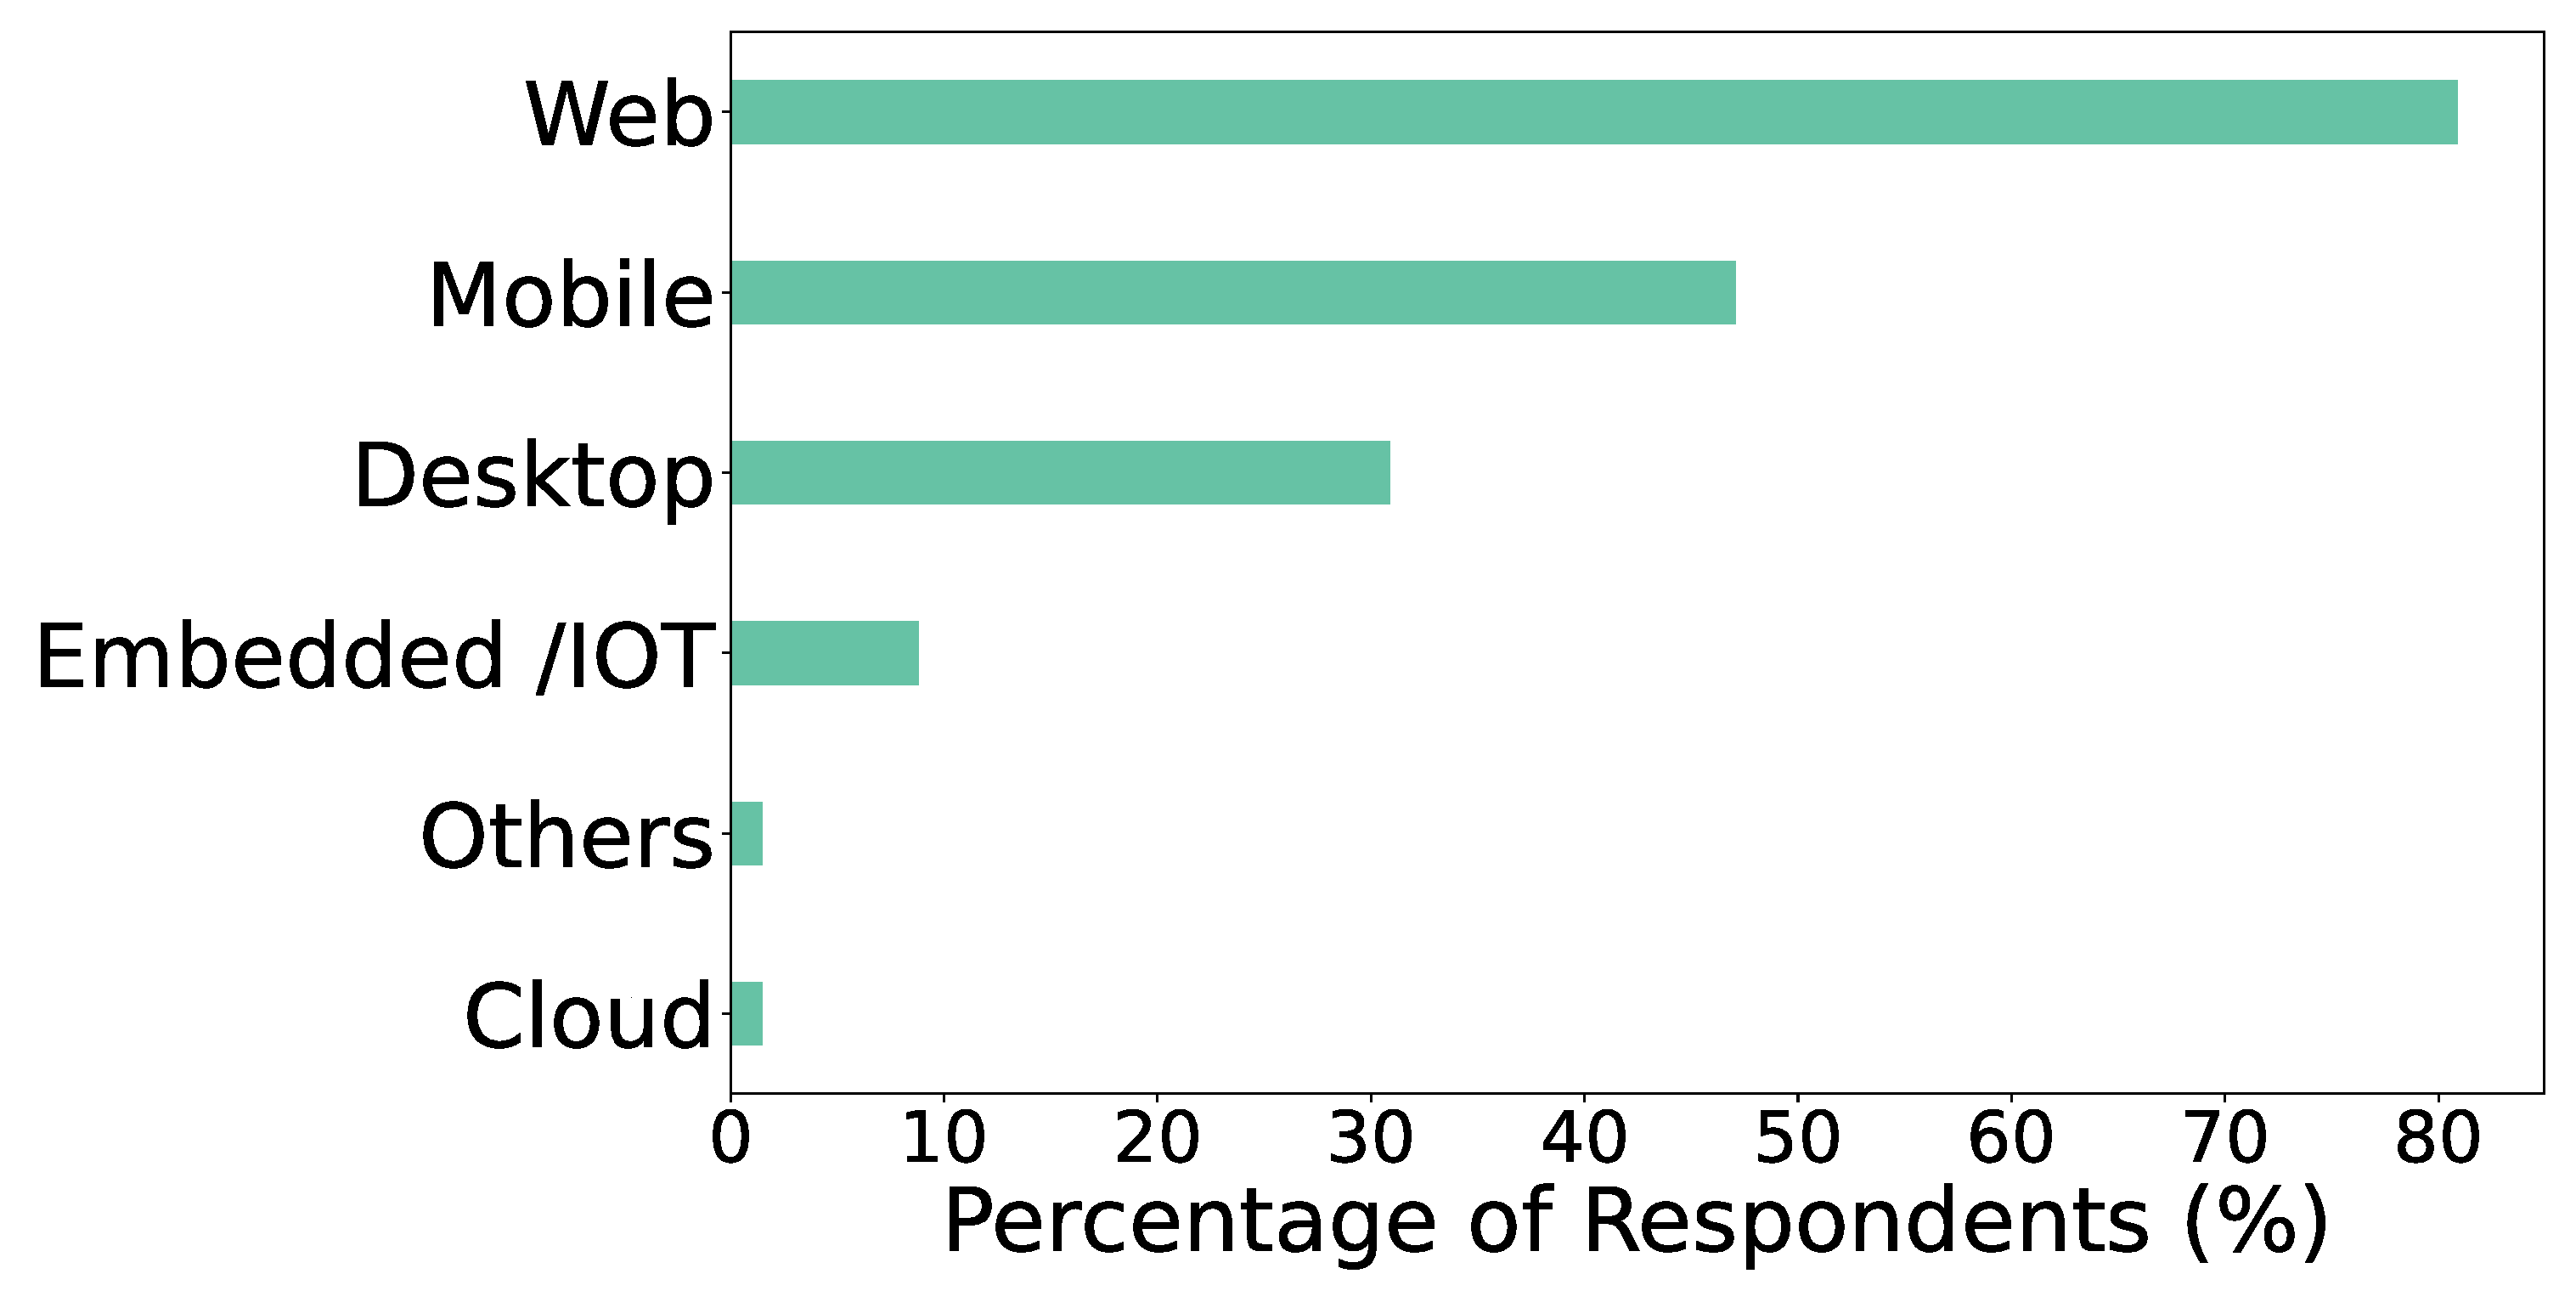
\includegraphics[scale=0.18]{Figures/Respondents_Technologies}
  \caption{Technology Platforms}
  \label{fig:platforms}
\end{figure}
\begin{figure}[t]
\centering
  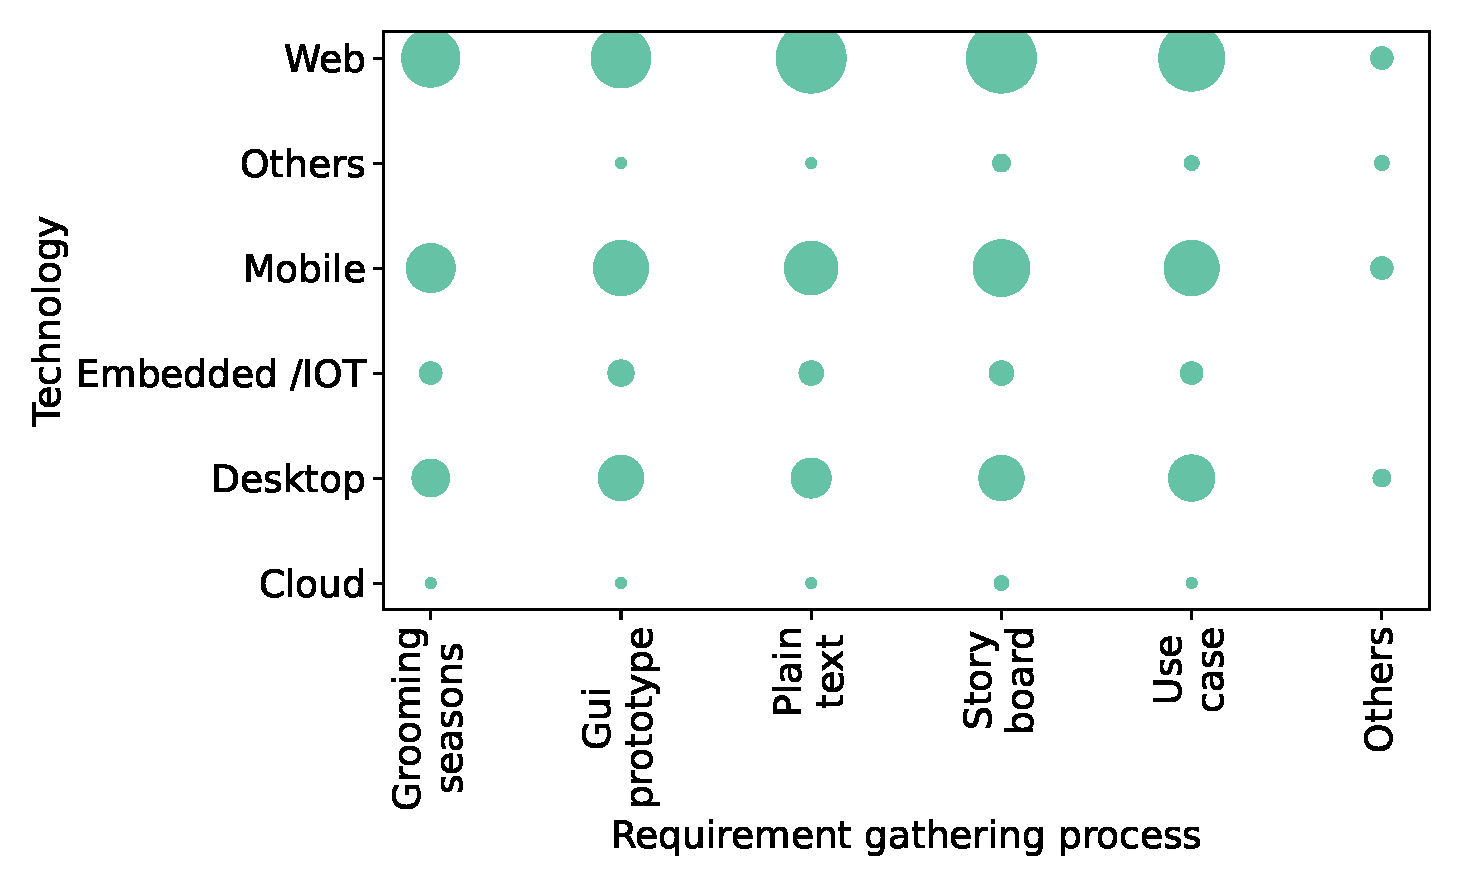
\includegraphics[scale=0.47]{Figures/Requirement_Technology_Cross_Analysis.eps}
  \caption{Cross aspect analysis of requirement gathering and technology platform}
  \label{fig:requirement technology cross analysis}
\end{figure}

%\paragraph{Operating Systems (Q10).} 

For operating systems (Q10), most of our
respondents preferred Linux based operating system (56\%) for their development (Figure \ref{fig:os}). The second frequently used
operating system is Windows (45\%) followed by MacOS (28\%). We
observed similar scenarios in the 2018 and 2019 StackOverflow (SO) surveys
\cite{StackoverflowSurvey2018,StackoverflowSurvey2019}. However, Windows ranked
first in the 2020 survey of both SO and JetBrains \cite{StackoverflowSurvey2020,
JetBrains2020}. The recent higher preference towards Windows could be due to the newly
included WSL (Windows Subsystem for Linux). This feature allows users to perform
almost any Linux-specific task on Windows. We anticipated that the use of OS
might be related to professional experience. Among the participants,
senior/expert developers (those with at least 5 years of experience) have significantly higher rates of Linux usage ($p=0.024$ based on Mann Whitney U test). 
\begin{figure}[h]
\centering
  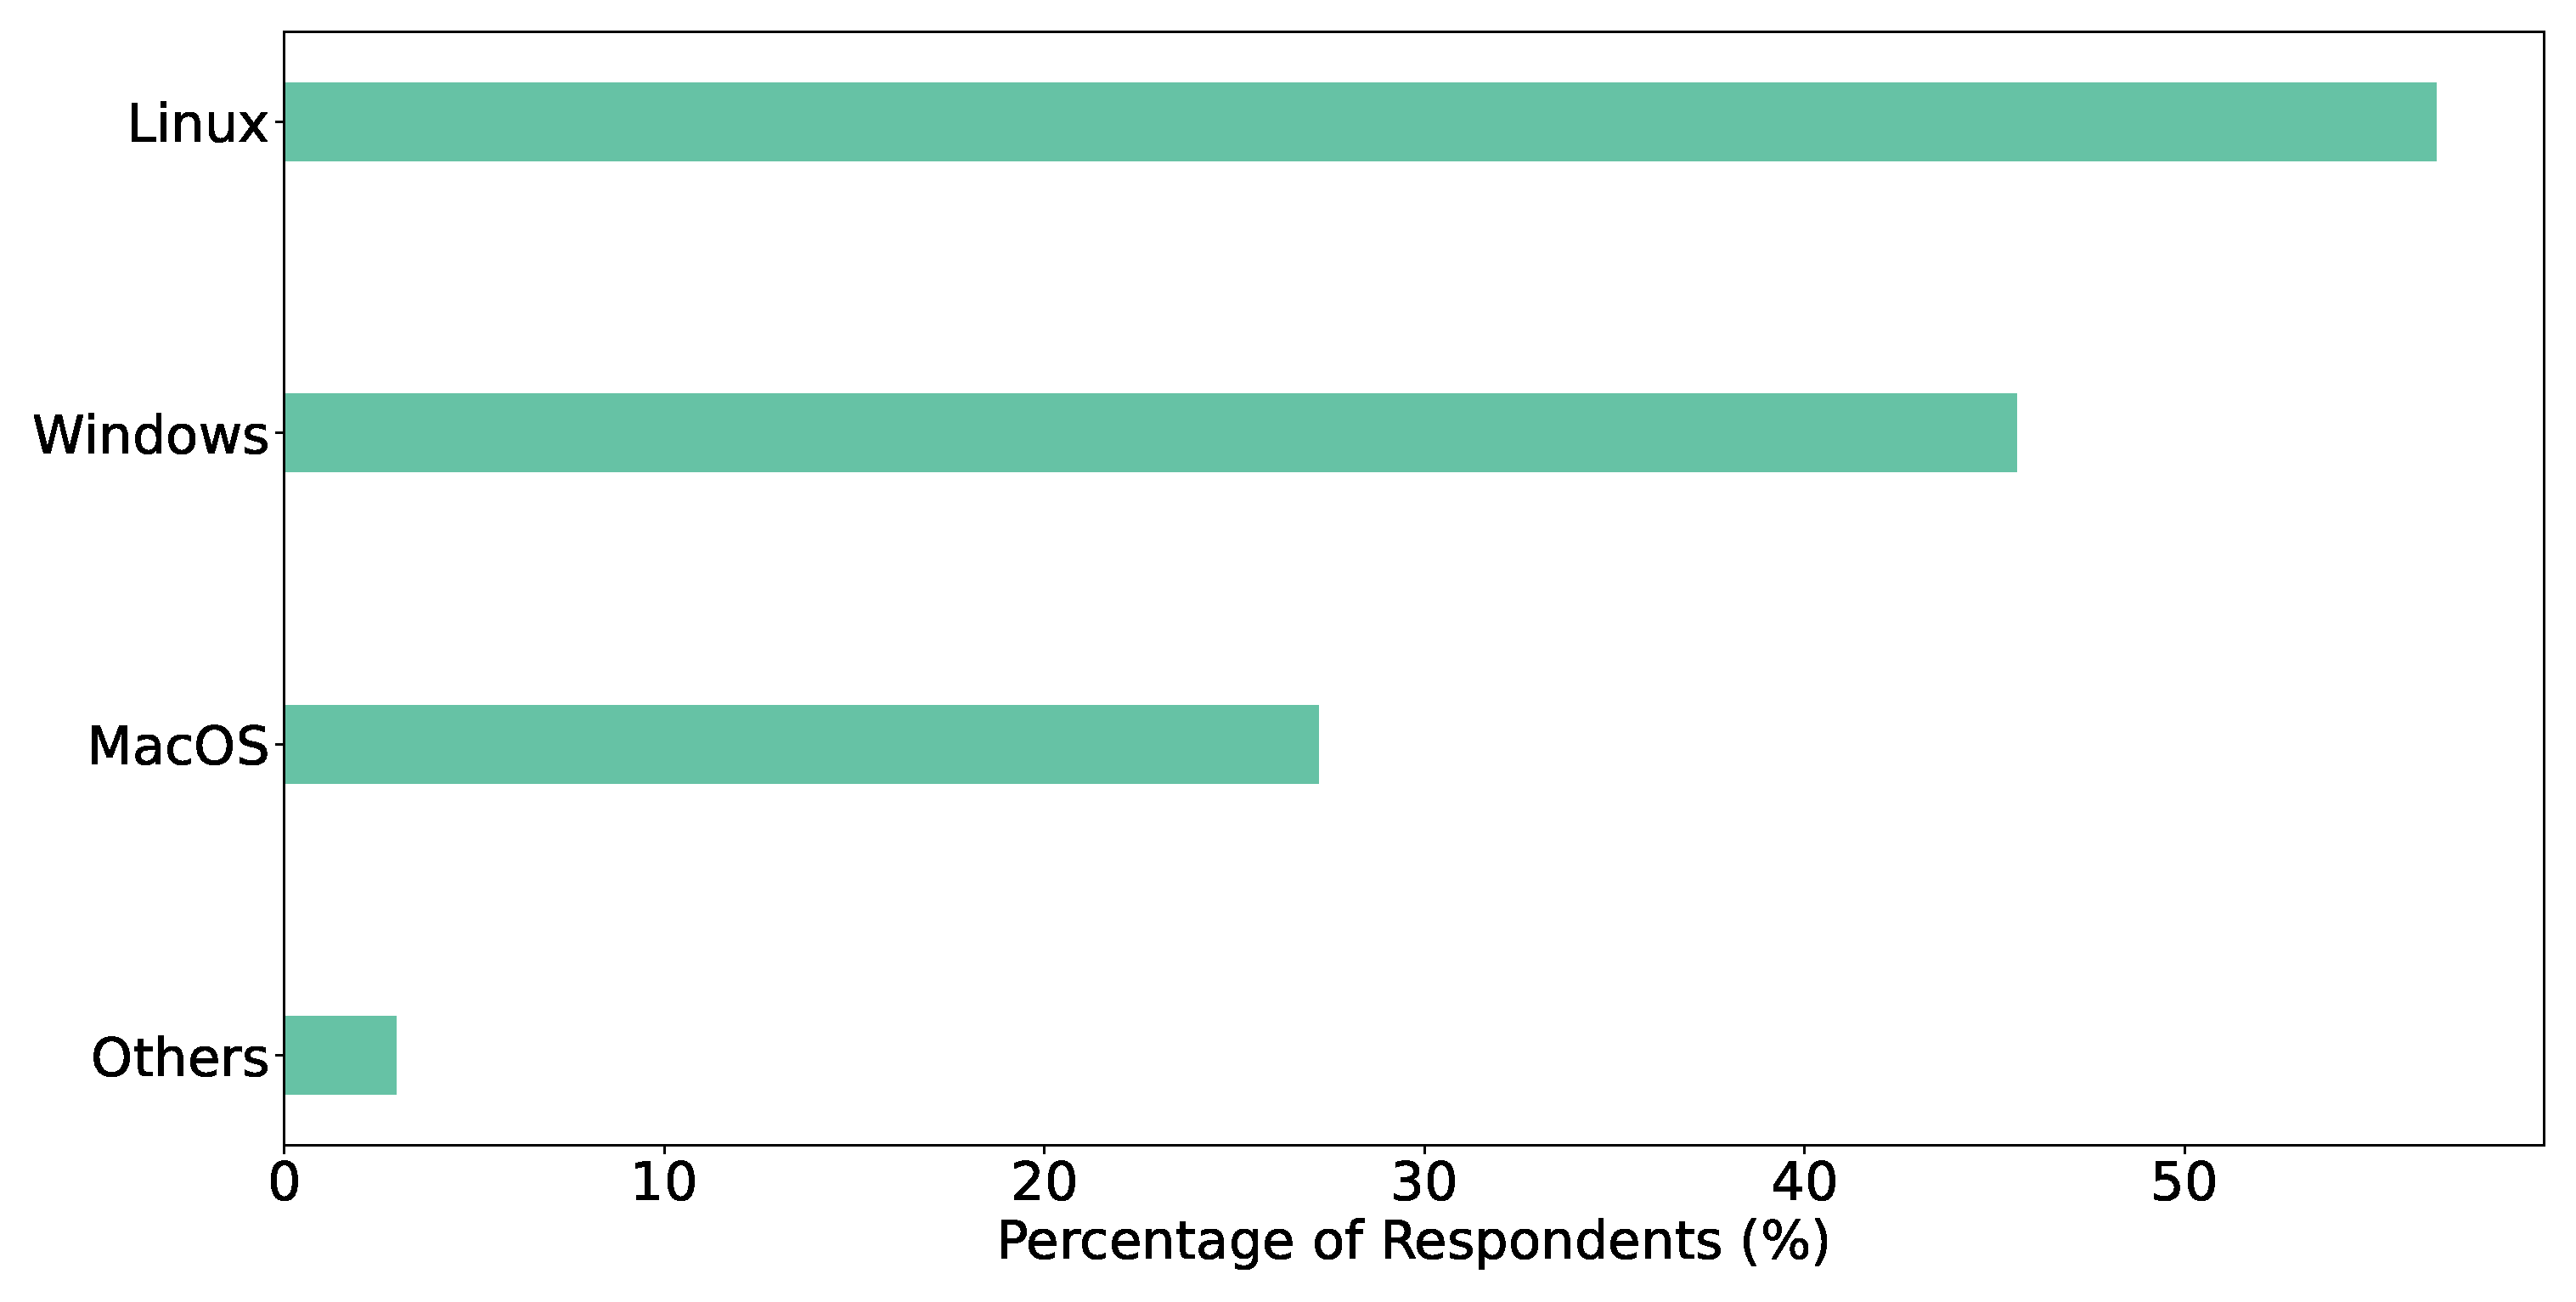
\includegraphics[scale=0.17]{Figures/Respondents_os}
  \caption{Operating Systems}
  \label{fig:os}
\end{figure}
%\paragraph{Programming Languages (Q11).} 
For programming languages (Q11), around 65\% and 60\% of our respondents use JavaScript and
Java, respectively, which are the two most used languages in Bangladesh (Figure
\ref{fig:languages}). Both JavaScript and Java are popular for web and mobile
platforms. A great percentage of our survey participants develop for both
web and mobile platforms. Other languages
like PHP (25\%), Python (25\%), and C\# (18\%) are also used, which indicates
that the software engineers are not biased towards a single specific language.
Our survey result matches with the last two years' Stack Overflow survey and the
GitHub stat. In all of the cases, JavaScript is the most used language, followed
by Java and Python \cite{StackoverflowSurvey2020, StackoverflowSurvey2019,
GithubStat}. We
observed that users using mobile and web platforms mostly use Java and
Javascript as programming languages. However, this is not statistically
significant ($p=0.1$). Though the use of the operating system can be influenced by
programming language (e.g., Swift and macOS), we do not find any significant correlation
between the two choices.
\begin{figure}[t]
\centering
  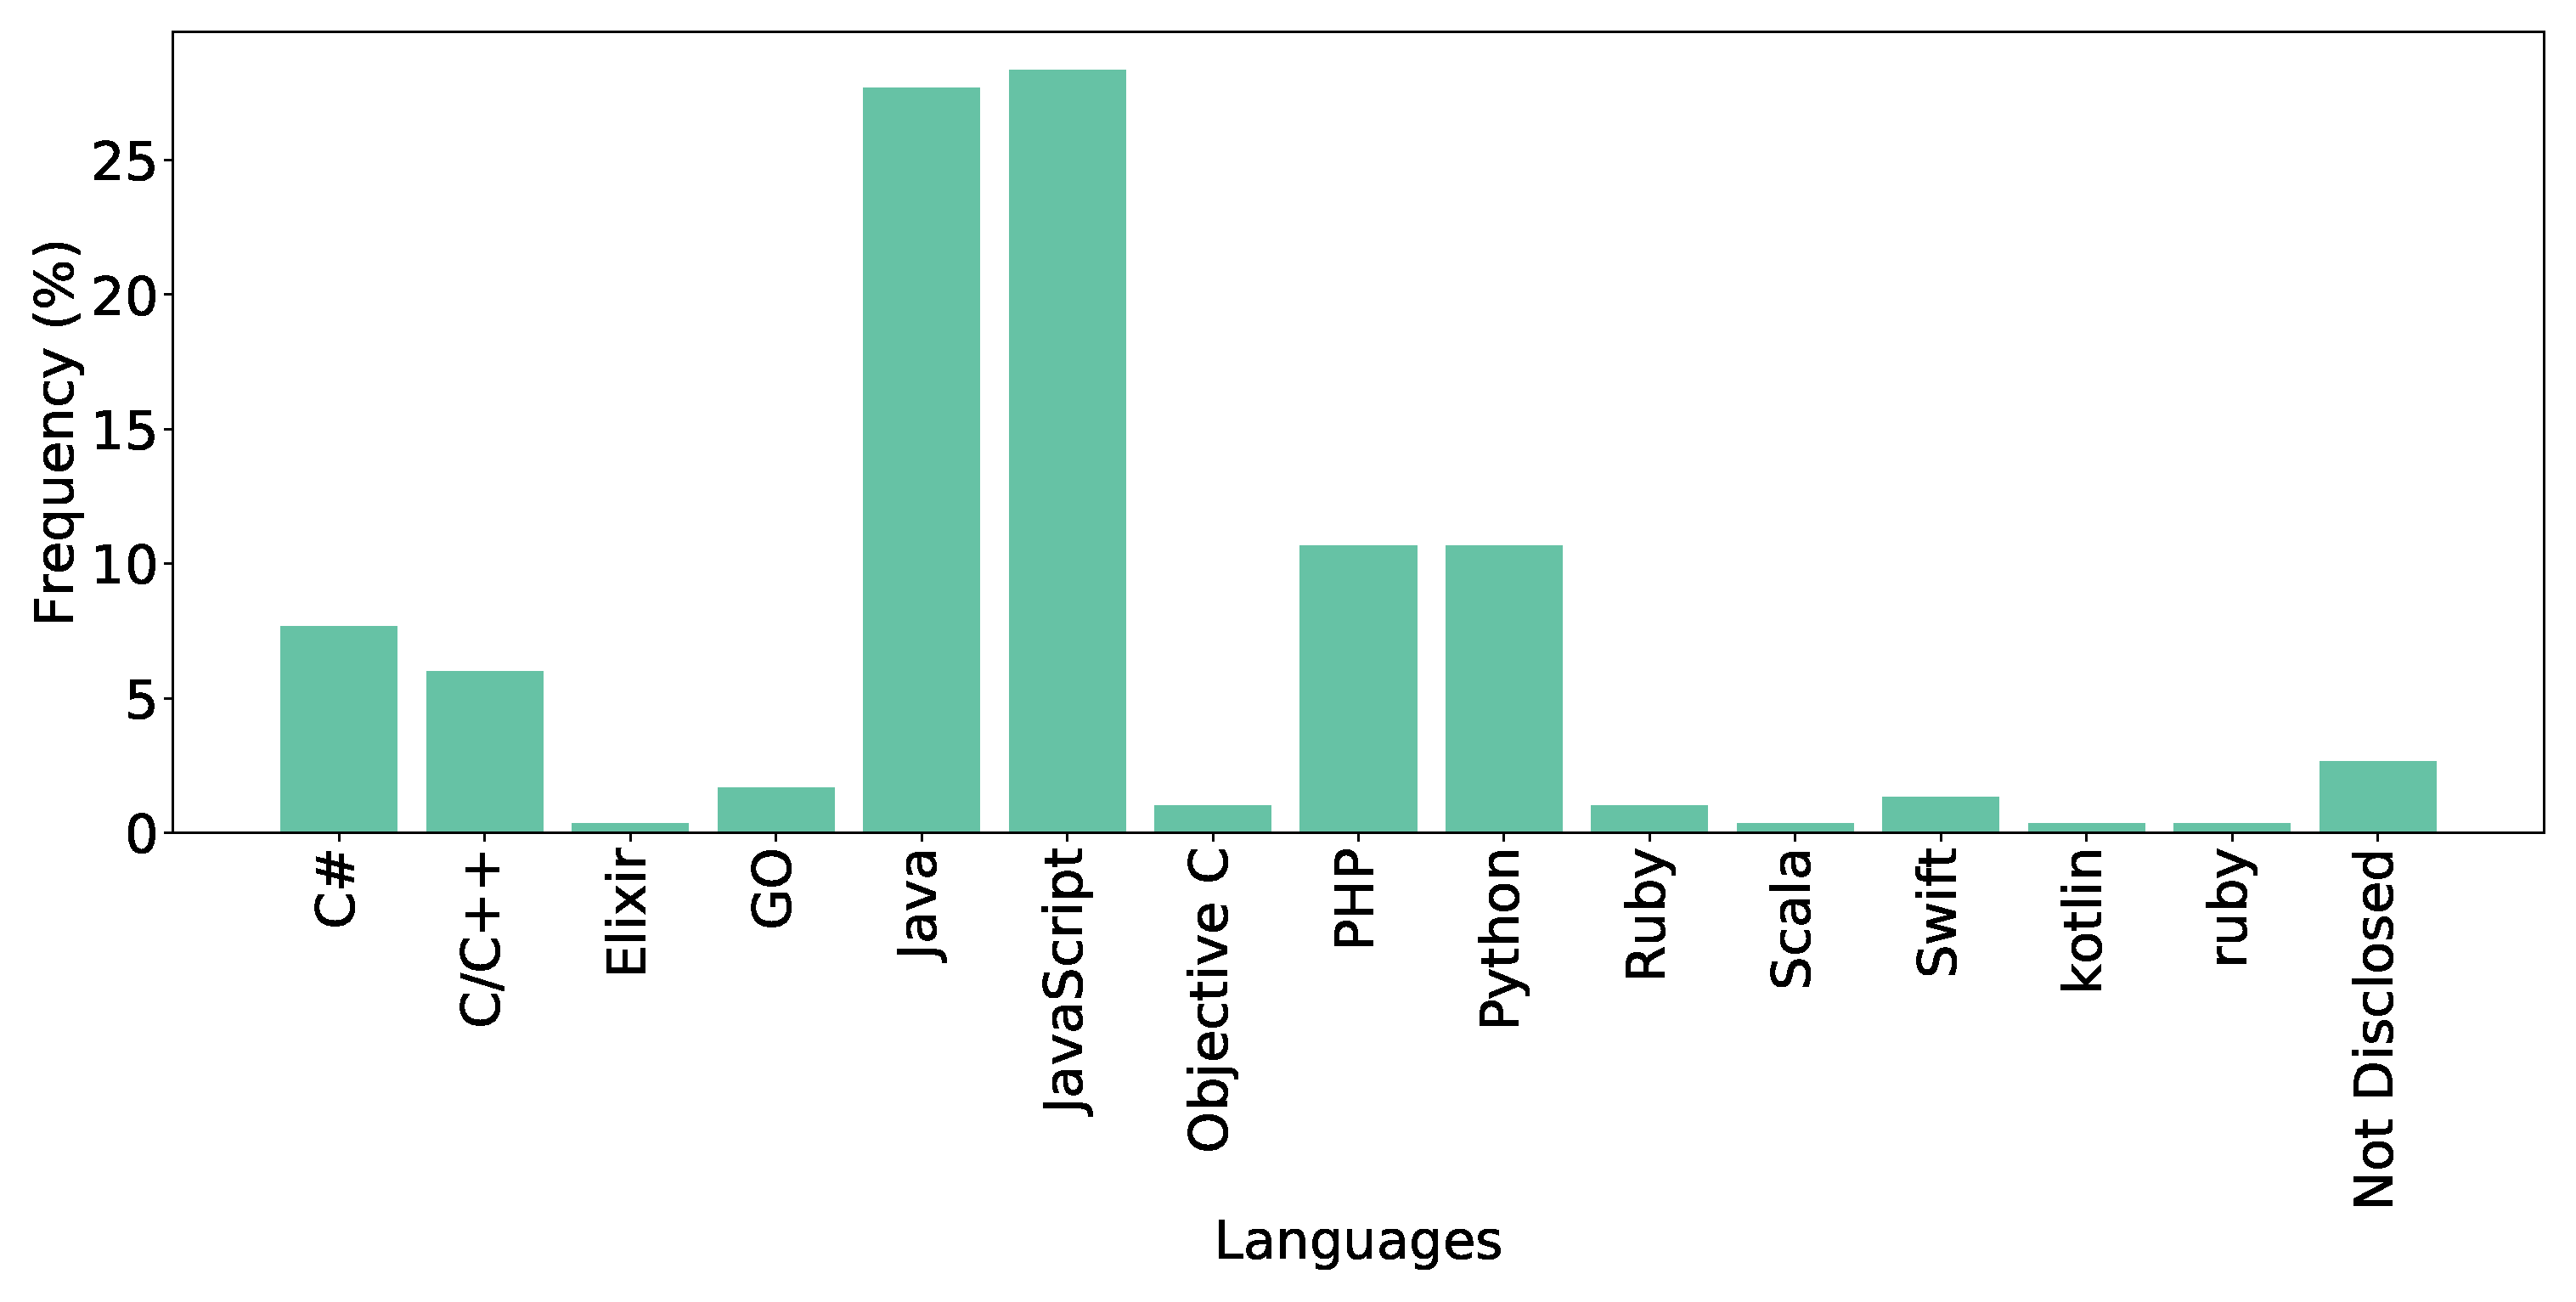
\includegraphics[scale=0.18]{Figures/Respondents_languages}
  \caption{Languages used in software development}
  \label{fig:languages}
\end{figure}

%\paragraph{Frameworks used in development}
For frameworkes used in development (Q12), as shown in Figure \ref{fig:frameworks} Spring boot (37\%) is the most used framework in the Bangladesh software industry. 
This observation is aligned with the result of Java's usage rate corresponding
to Figure \ref{fig:languages}. Since JavaScript is the most used language of our
respondents, they use various JavaScript frameworks such as React, Node.js,
Angular, Express, etc. ASP.NET, Django, and
Laravel are used in the same proportion based on around 15\% of our respondents.
React, Swift, Ruby on Rails, Node.js, etc., are comparatively less used. Other
than these, lots of frameworks such as Cocoa, Meteor, TestNG, Relay, Appium,
CakePHP, etc., are also used (presented as `Others' in Figure \ref{fig:frameworks}). For web development, Django
and Spring frameworks are mostly used in Bangladesh ($p=0.04$). We have compared
our results with the Stack Overflow 2016 to 2020
survey\cite{StackoverflowSurvey2017, StackoverflowSurvey2018,
StackoverflowSurvey2019, StackoverflowSurvey2020}. The only common framework in
the top five list in both surveys is ASP.NET. In the stack overflow survey, we
noticed that JavaScript-based frameworks (e.g., Jacqueline, Angular, React,
Node.js) occupy the top positions (top five), which is not the case for our
survey.

\begin{figure}[t]
\centering
  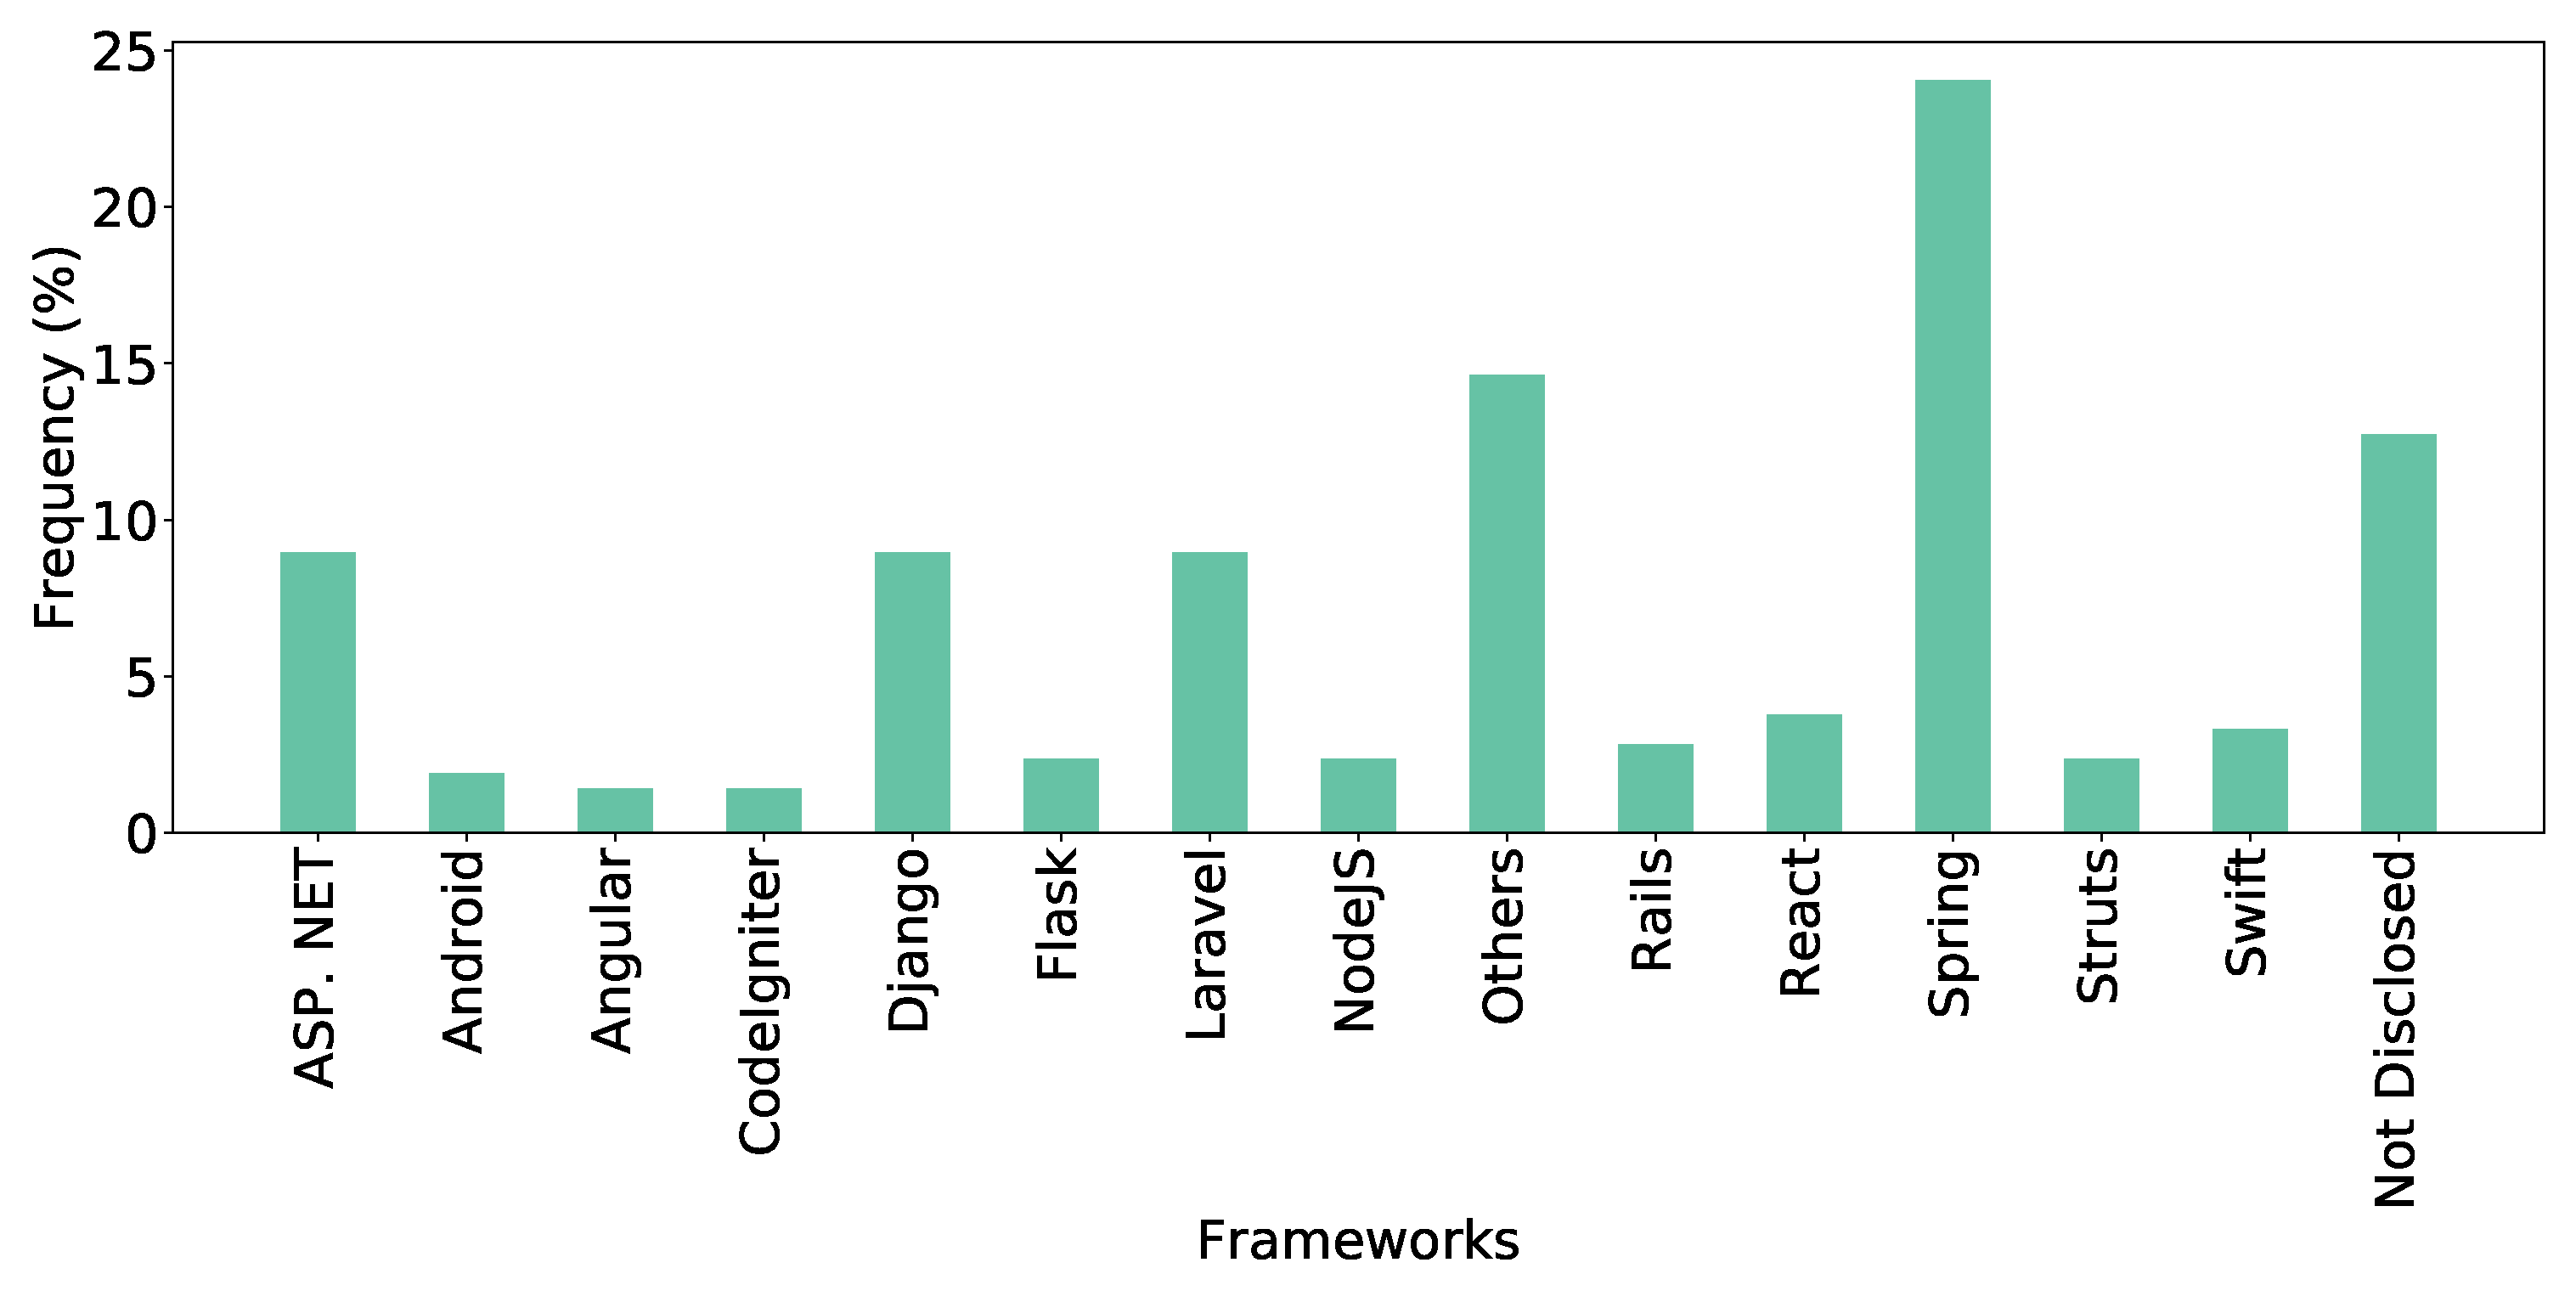
\includegraphics[scale=0.18]{Figures/Respondents_frameworks}
  \caption{Frameworks}
  \label{fig:frameworks}
\end{figure}

%\paragraph{IDE's used by the respondent's} 
Among the IDEs (Q13), as shown in Figure \ref{fig:IDEs},
IntelliJ, is used by most respondents (43\%). IntelliJ is a Java integrated development tool for developing software for the
enterprise, mobile, and web application, The
other IDEs used in SE industries are Visual Studio (30\%), Eclipse (24\%),
PyCharm (17\%), NetBeans (11\%), and Android Studio (7\%).

\begin{figure}[t]
\centering
  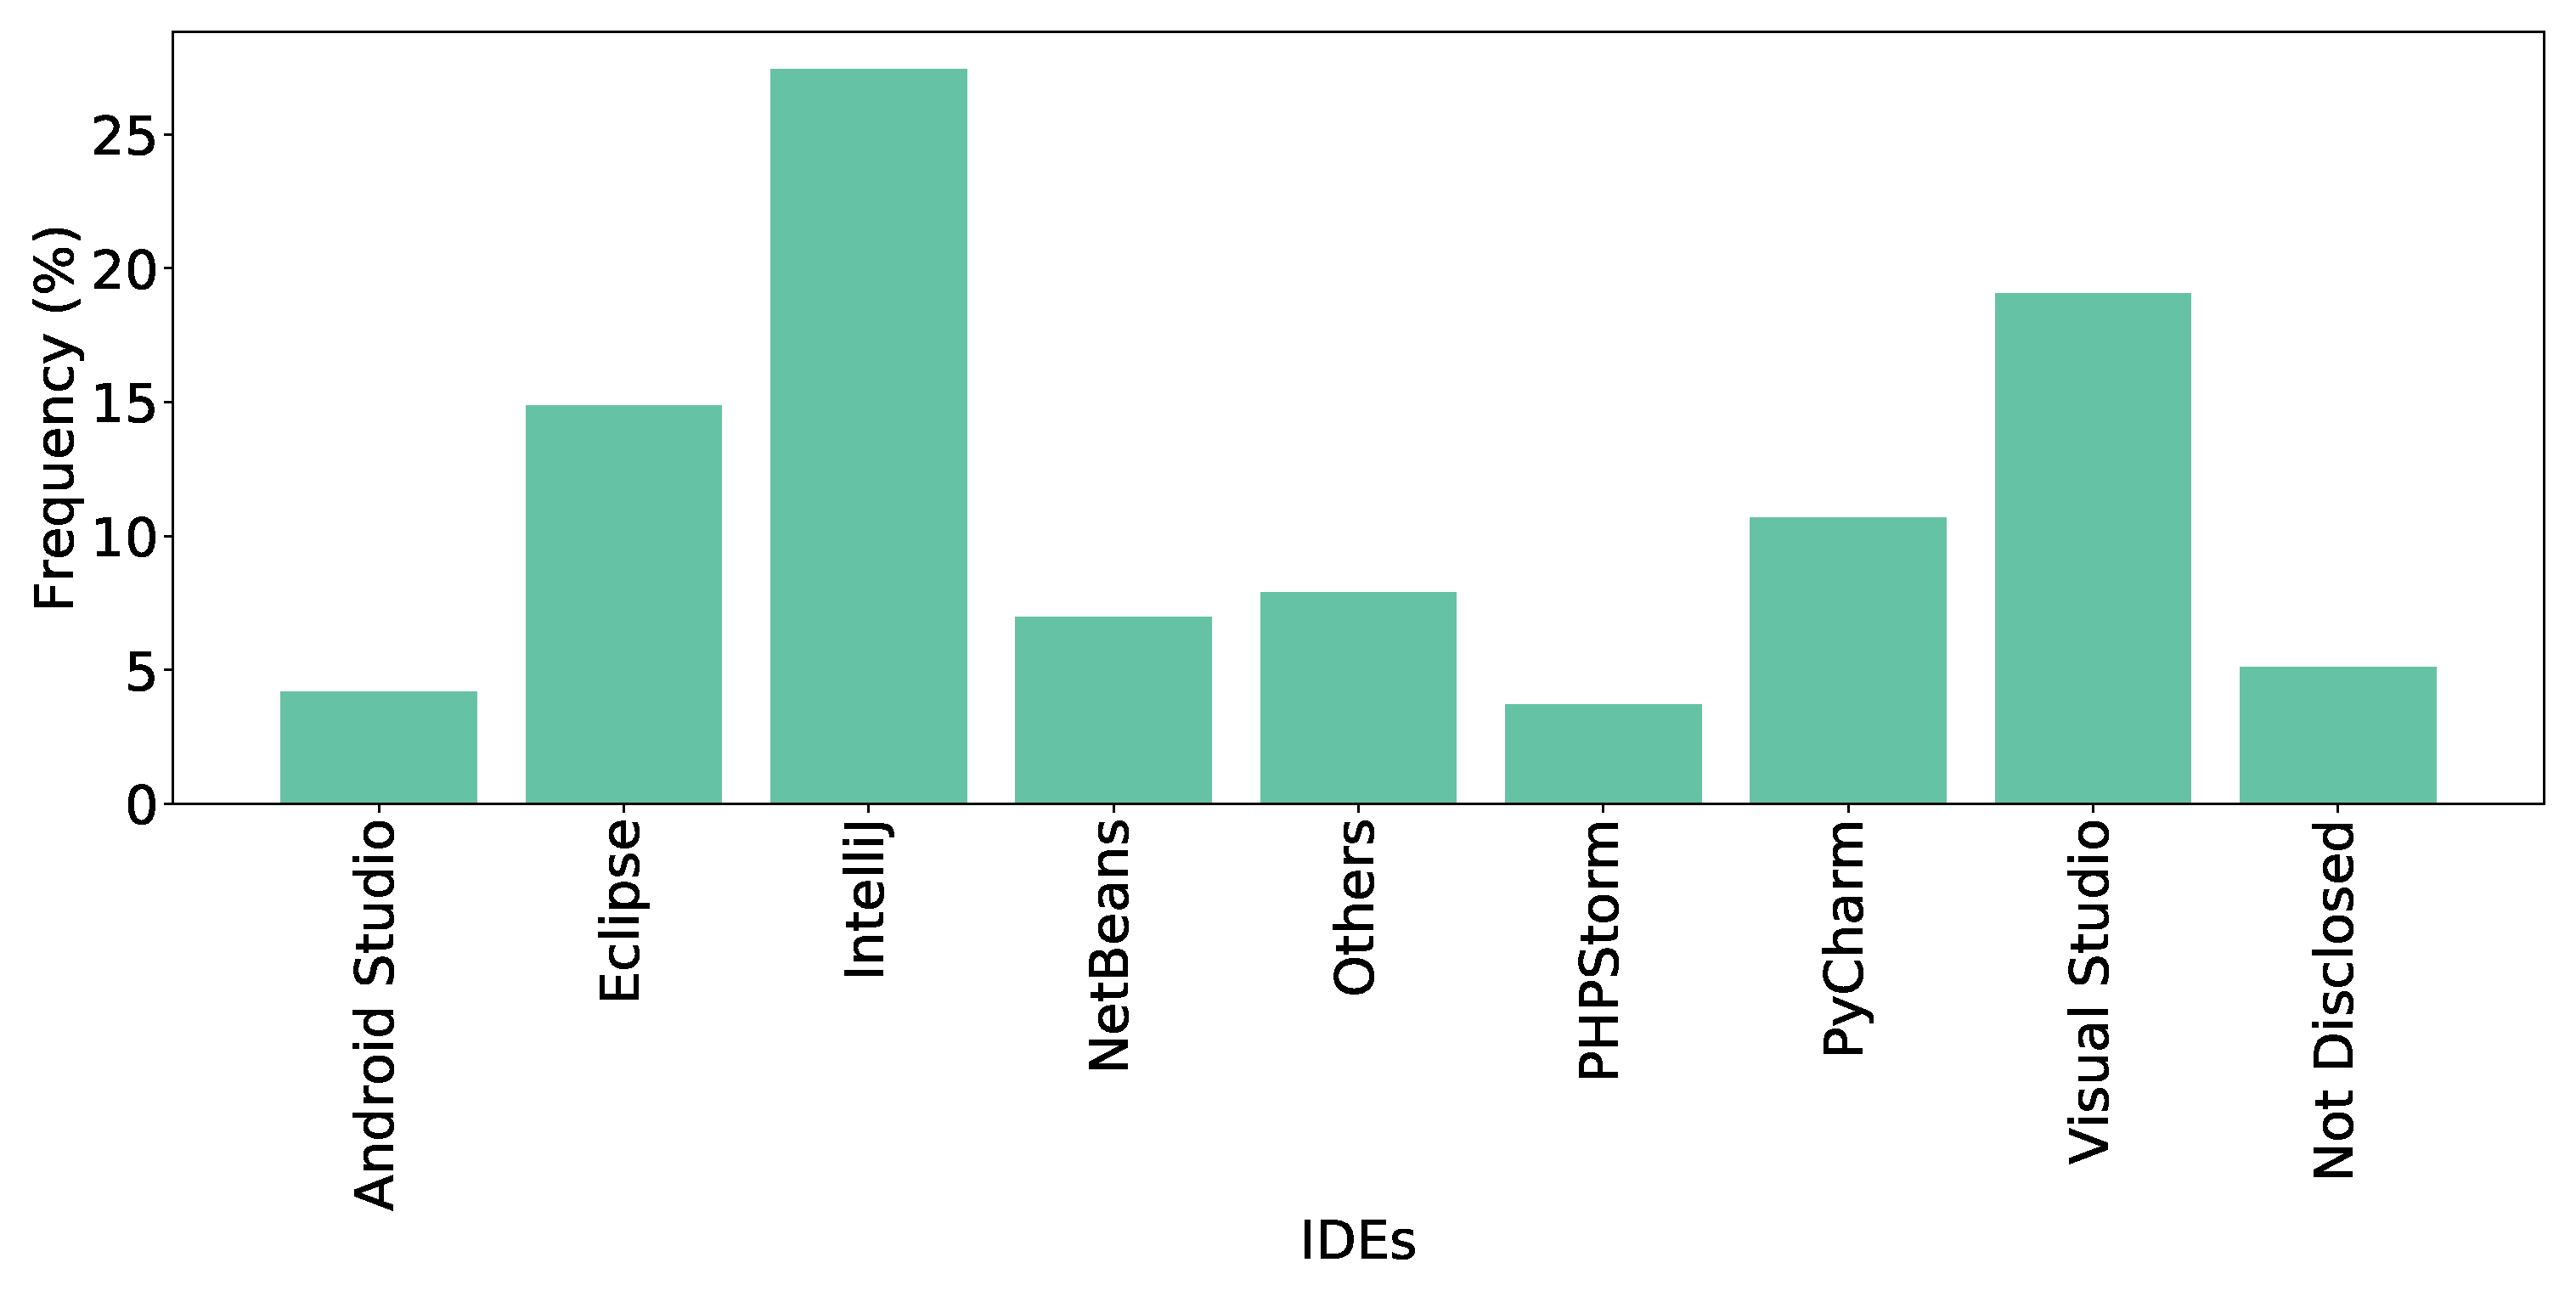
\includegraphics[scale=0.18]{Figures/Respondents_IDEs}
  \caption{IDE's}
  \label{fig:IDEs}
\end{figure}
\begin{tcolorbox}[flushleft upper,boxrule=1pt,arc=0pt,left=0pt,right=0pt,top=0pt,bottom=0pt,colback=white,after=\ignorespacesafterend\par\noindent]
\nd\it{\bf{RQ1-D2. Software development tools and techniques used.}} Web based software services top the list of development technologies. Requirement gathering process is mostly practiced in GUI-based development
(e.g., web, desktop, mobile) \gias{summarize findings from Q10-13 also here}
\end{tcolorbox}
% \boxtext{Web based software services top the list of development technologies. Requirement gathering process is mostly practiced in GUI-based development
% (e.g., web, desktop, mobile) \gias{summarize findings from Q10-13 also here}}
